\documentclass[11pt,a4paper]{article}
\usepackage[utf8]{inputenc}
\usepackage{amsmath,amssymb,amsfonts}
\usepackage{graphicx}
\usepackage{booktabs}
\usepackage{geometry}
\usepackage{hyperref}
\usepackage{float}
\geometry{margin=1in}

\title{\textbf{Krylov Subspace Diagonalization vs. Standard Trotterization for 1D Ring XXZ Hamiltonians on NISQ Devices}}
\author{Hyunwoo Choi}
\date{\today}

\begin{document}

\maketitle

\begin{abstract}
Lattice Hamiltonians simulation on Noisy Intermediate-Scale Quantum (NISQ) computers faces severe challenges due to deep circuit requirements. In this report, we evaluate and compare the standard Trotterization time-evolution method and the Krylov Quantum Diagonalization (KQD) method on a 1D ring XXZ Hamiltonian with 4 qubits. We demonstrate that KQD drastically reduces the circuit depth and 2-qubit gate count compared to standard Trotterization. We further investigate the trade-off between Trotter step count and KQD convergence quality, analyze the standard Trotterization dynamics via classical FFT to extract energy spectra without Quantum Phase Estimation, and quantify the mathematical source of unphysical values below the variational lower bound.
\end{abstract}

\section{Introduction}
Simulating the time evolution of quantum spin systems, such as the XXZ model, is a primary application of quantum computing. However, standard deterministic Trotterization methods require deep circuits for long time evolutions, leading to a rapid accumulation of gate errors on NISQ devices. This report examines the Krylov Quantum Diagonalization (KQD) algorithm, a subspace method that constructs an effective Hamiltonian within a small Krylov subspace generated by short real-time evolutions, and compares it directly with standard Trotterization using both quantum simulation data and classical FFT post-processing.

\section{Theoretical Background}
\subsection{Krylov Quantum Diagonalization (KQD)}
The unitary Krylov subspace of dimension $r$ is spanned by the state vectors:
\begin{equation}
\mathcal{K}_U^r = \{ |\psi\rangle, U(dt)|\psi\rangle, \dots, U((r-1)dt)|\psi\rangle \}
\end{equation}
where $U(dt) = e^{-i H dt}$. To find the ground state energy within this subspace, we solve the generalized eigenvalue problem:
\begin{equation}
\tilde{H} \vec{c} = E \tilde{S} \vec{c}
\end{equation}
where $\tilde{H}_{mn} = \langle \psi_m | H | \psi_n \rangle$ and $\tilde{S}_{mn} = \langle \psi_m | \psi_n \rangle$.

\subsection{Efficient Hadamard Test}
Using the U(1) symmetry of the XXZ Hamiltonian, the vacuum state $|0\rangle^N$ is an eigenstate: $U(t)|0\rangle^N = e^{-i E_0 t}|0\rangle^N$. This allows the substitution of controlled time evolution with uncontrolled evolution, yielding a shallow Hadamard test circuit.

\subsection{Classical FFT Analysis of Time-Domain Data}
Given time-domain expectation values $\langle Z_0(t) \rangle$ from standard Trotterization, the energy transition frequencies can be extracted classically via a discrete Fourier transform without Quantum Phase Estimation (QPE). The observable decomposes as:
\begin{equation}
\langle Z_0(t) \rangle = \sum_{k,l} c_k^* c_l \langle k | Z_0 | l \rangle \, e^{-i(E_l - E_k)t}
\end{equation}
where $c_k = \langle k | \psi \rangle$ are the initial state overlaps. The FFT power spectrum thus reveals peaks at transition frequencies $\omega_{kl} = |E_l - E_k|$.

\section{Methodology}
We configure a 1D ring XXZ Hamiltonian:
\begin{equation}
H = \sum_{\langle i,j \rangle} (X_i X_j + Y_i Y_j + 0.5 Z_i Z_j) + 0.5 \sum_i Z_i
\end{equation}
on $N=4$ qubits with periodic boundary conditions. The reference state is the Neel state $|\psi\rangle = |1010\rangle$.
The Krylov dimension is set to $r=5$. The time step $dt$ is computed using the spectral norm of the single-excitation subspace Hamiltonian: $dt = \pi / ||H_{single}||_2 \approx 0.6283$.

An adaptive error mitigation routine is implemented:
\begin{itemize}
    \item If $depth < 80$ and $2Q\_gates < 100$: Enable ZNE, DD, and TREX.
    \item Otherwise: Disable ZNE, keep DD and TREX.
\end{itemize}

\section{Results and Comparison}

\subsection{Circuit Complexity Comparison}
We compare the transpiled circuits for standard Trotterization and KQD on noiseless (\texttt{AerSimulator}) and noisy device (\texttt{FakeBrisbane}) backends.

\begin{table}[H]
\centering
\caption{Transpiled Circuit Metrics Comparison (Standard Trotter: $t=2.0$, 10 steps, Suzuki-2; KQD: $r=5$, 2-step, Lie)}
\begin{tabular}{lcccccc}
\toprule
Method & Backend & Qubits & Depth & 2Q Gates & ZNE Status \\
\midrule
Std Trotter ($t=0.1$) & \texttt{AerSimulator} & 4 & 20 & 24 & Enabled \\
Std Trotter ($t=2.0$) & \texttt{AerSimulator} & 4 & 191 & 240 & Disabled \\
KQD (2-step) & \texttt{AerSimulator} & 5 & 24 & 28 & Enabled \\
\midrule
Std Trotter ($t=0.1$) & \texttt{FakeBrisbane} & 127 & 114 & 27 & Disabled \\
Std Trotter ($t=2.0$) & \texttt{FakeBrisbane} & 127 & 970 & 243 & Disabled \\
KQD (2-step) & \texttt{FakeBrisbane} & 127 & 317 & 59 & Enabled \\
\bottomrule
\end{tabular}
\end{table}

\subsection{KQD Trotter Steps vs. Circuit Depth Trade-off}
Increasing the number of Trotter steps in the KQD template circuit improves the accuracy of the Trotterized time-evolution operator, but at the cost of deeper circuits. The following table and Figure~\ref{fig:kqd_circuit_metrics} quantify this trade-off on the noiseless \texttt{AerSimulator}.

\begin{table}[H]
\centering
\caption{KQD Circuit Metrics vs. Trotter Steps (\texttt{AerSimulator})}
\begin{tabular}{cccc}
\toprule
Trotter Steps & $\Delta t$ (step size) & Depth & 2Q Gates \\
\midrule
1 & 0.6283 & 17 & 16 \\
2 & 0.3142 & 24 & 28 \\
4 & 0.1571 & 38 & 52 \\
6 & 0.1047 & 52 & 76 \\
\bottomrule
\end{tabular}
\end{table}

\begin{figure}[H]
\centering
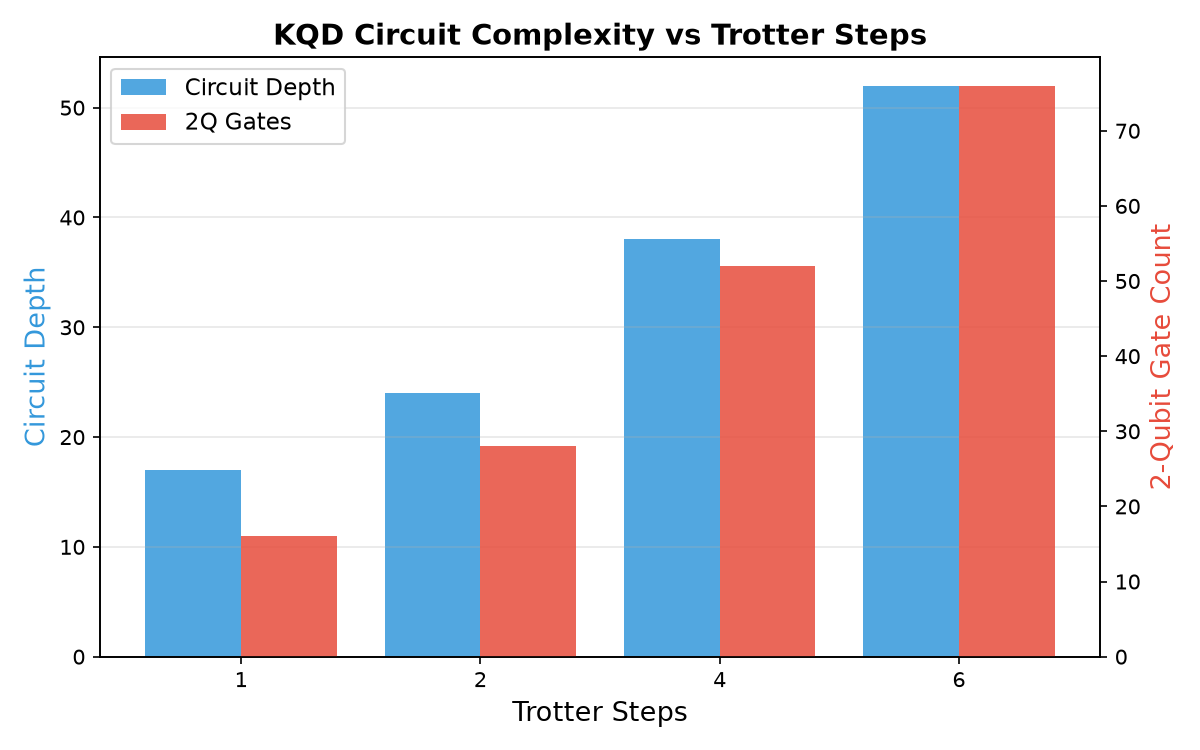
\includegraphics[width=0.75\textwidth]{kqd_circuit_metrics.png}
\caption{KQD circuit depth and 2-qubit gate count as a function of Trotter steps.}
\label{fig:kqd_circuit_metrics}
\end{figure}

\subsection{KQD Energy Convergence vs. Trotter Steps}
Figure~\ref{fig:kqd_trotter_sweep} shows the KQD ground state energy estimate as a function of Krylov dimension $d$ for different numbers of Trotter steps on the noiseless backend. The exact ground state energy is $E_{exact} = -6.744563$.

\begin{figure}[H]
\centering
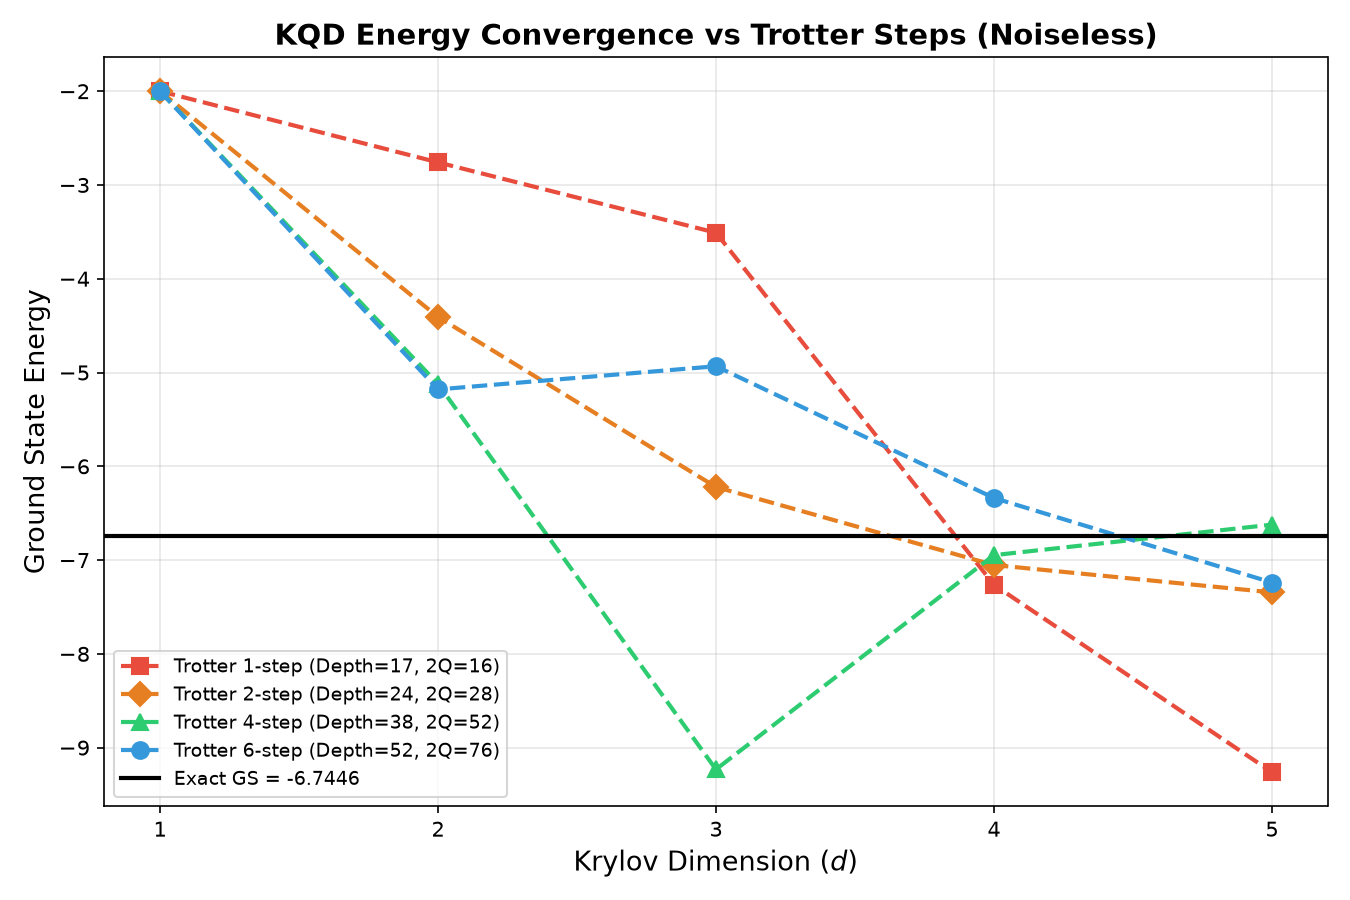
\includegraphics[width=0.85\textwidth]{kqd_trotter_sweep_energy.png}
\caption{KQD energy convergence for different Trotter step counts. With 1-step Trotter, the energy diverges to $-9.26$ at $d=5$ due to extreme Trotter error. Higher step counts show stable convergence toward the exact ground state, albeit at the cost of deeper circuits. Note that the 4-step case shows anomalous behavior at $d=3$ (overshoot to $-9.23$), likely due to numerical conditioning of the $S$ matrix at that particular subspace dimension.}
\label{fig:kqd_trotter_sweep}
\end{figure}

\subsection{Variational Principle Violation}
This apparent violation of the variational principle (obtaining energies below $E_{exact}$) originates from the non-commutativity of the Trotterized evolution operator $U_{Trotter}(t)$ and the Hamiltonian $H$.
In the KQD matrix reconstruction, the elements are approximated as $\tilde{H}_{mn} = \langle \psi | H U_{Trotter}((n-m)dt) | \psi \rangle$, assuming $U_{Trotter}^\dagger(t_m) H U_{Trotter}(t_n) = H U_{Trotter}^\dagger(t_m) U_{Trotter}(t_n)$. Since $[H, U_{Trotter}] \neq 0$, the reconstructed matrix $\tilde{H}$ is no longer strictly of the variational projection form $V^\dagger H V$. As a result, the mathematical guarantee of the variational lower bound $E \geq E_{exact}$ is broken. Reducing the step size $\Delta t$ by increasing the number of Trotter steps restores this commutativity approximation, resolving the unphysical divergence.

\subsection{Standard Trotterization: Spin Dynamics and Classical FFT Analysis}
Rather than employing Quantum Phase Estimation (QPE), which would require prohibitively deep circuits on NISQ devices, we analyze the standard Trotterization time-domain data $\langle Z_0(t) \rangle$ using a classical discrete Fourier transform to extract energy transition frequencies.

\begin{figure}[H]
\centering
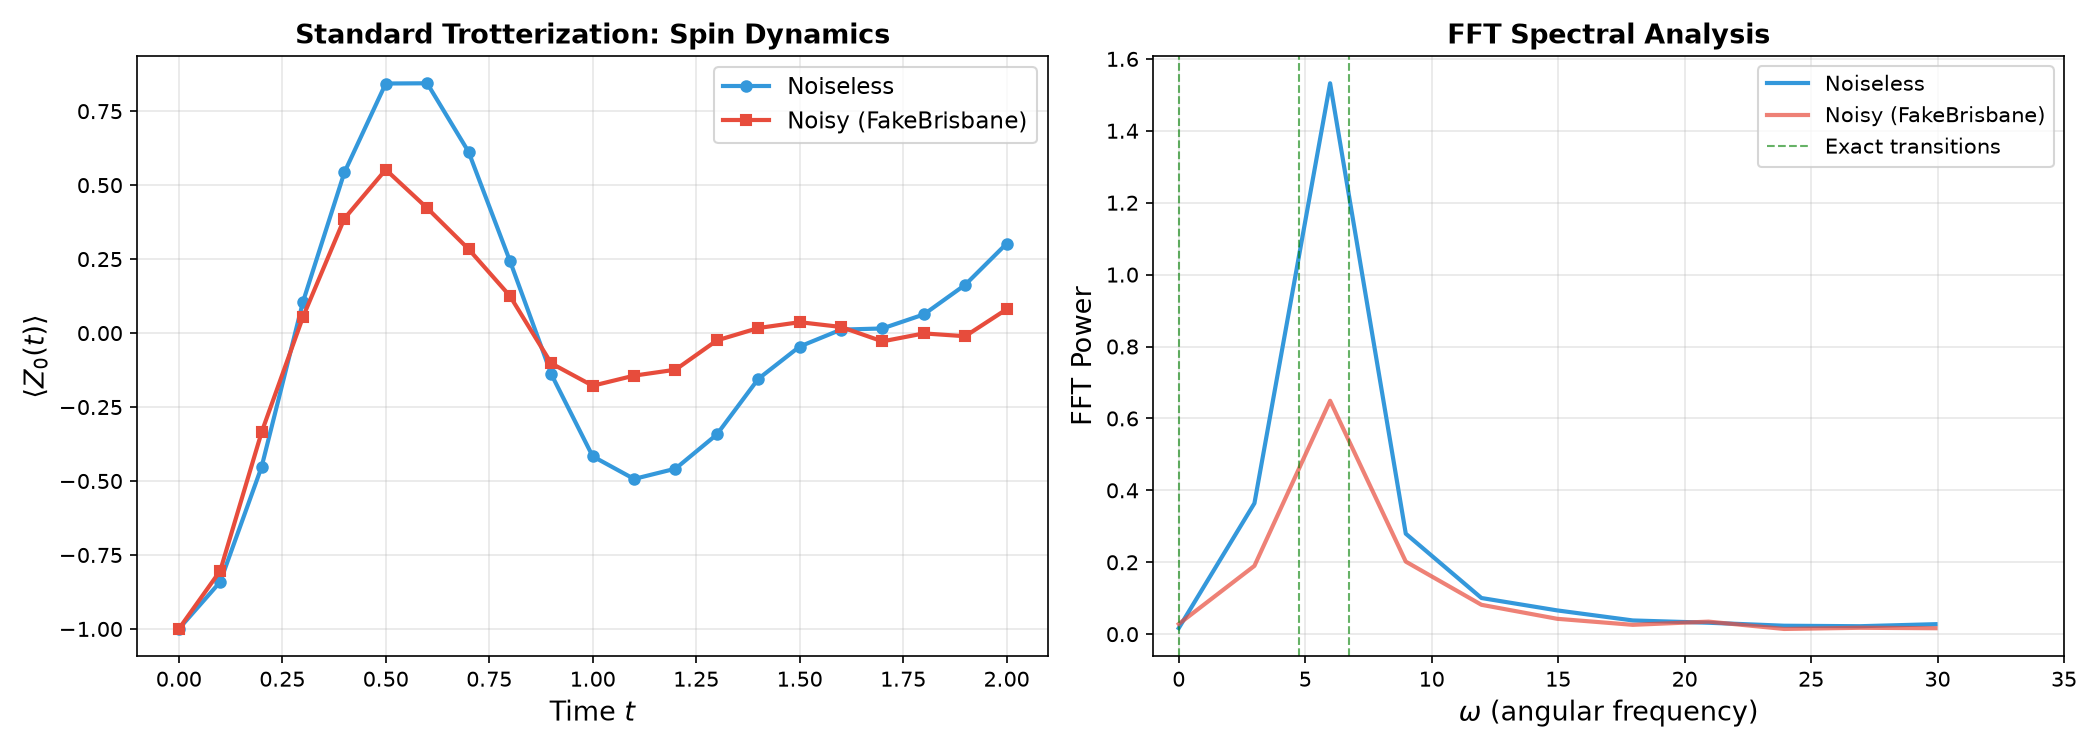
\includegraphics[width=\textwidth]{std_fft_analysis.png}
\caption{\textbf{Left:} Time-domain spin dynamics $\langle Z_0(t) \rangle$ under standard Trotterization. The noiseless (blue) signal oscillates with full amplitude, while the noisy FakeBrisbane (red) signal exhibits rapid damping. \textbf{Right:} FFT power spectrum. The dominant peak at $\omega \approx 5.98$ corresponds closely to the exact transition $|E_3 - E_0| = 4.74$ (green dashed), with additional harmonics visible. The noisy signal retains the same peak structure but with reduced power due to decoherence.}
\label{fig:fft_analysis}
\end{figure}

The FFT analysis reveals two key observations:
\begin{enumerate}
    \item The dominant FFT peak at $\omega \approx 5.98$ corresponds to the principal energy transition involving the Neel state decomposition coefficients. The exact Hamiltonian has eigenvalues $E_0 = -6.745$, $E_1 = -5.000$, $E_2 = -3.000$, $E_3 = -2.000$, ..., and the strongest transition from the Neel state occurs between $E_0$ and $E_3$, giving $\omega_{03} = |E_3 - E_0| = 4.745$.
    \item The noisy FakeBrisbane data retains the same spectral peaks but with reduced power, confirming that the oscillation frequencies are preserved even under noise, while amplitudes are damped. This demonstrates that classical FFT can extract useful spectral information from NISQ simulation data without deep QPE circuits.
\end{enumerate}

\subsection{KQD Noiseless Convergence (Updated, 6-step)}
Figure~\ref{fig:kqd_noiseless} shows the updated KQD convergence plot with 6-step Trotter on the noiseless simulator.

\begin{figure}[H]
\centering
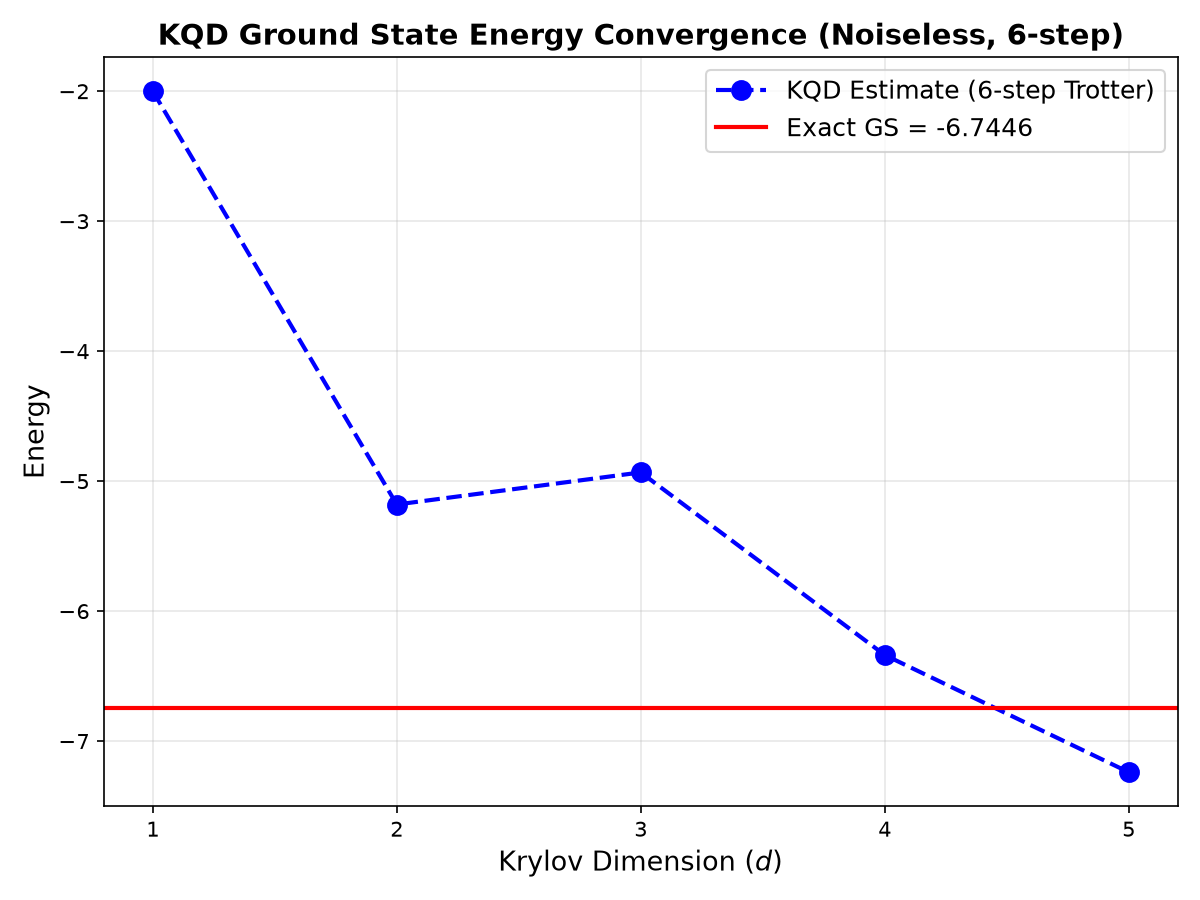
\includegraphics[width=0.7\textwidth]{kqd_convergence_noiseless.png}
\caption{KQD ground state energy convergence on the noiseless simulator (6-step Lie Trotter). The energy converges to approximately $-7.24$ at $d=5$, overshooting the exact value of $-6.7446$ slightly due to remaining Trotter error.}
\label{fig:kqd_noiseless}
\end{figure}

\subsection{KQD Noisy Convergence (FakeBrisbane)}
\begin{figure}[H]
\centering
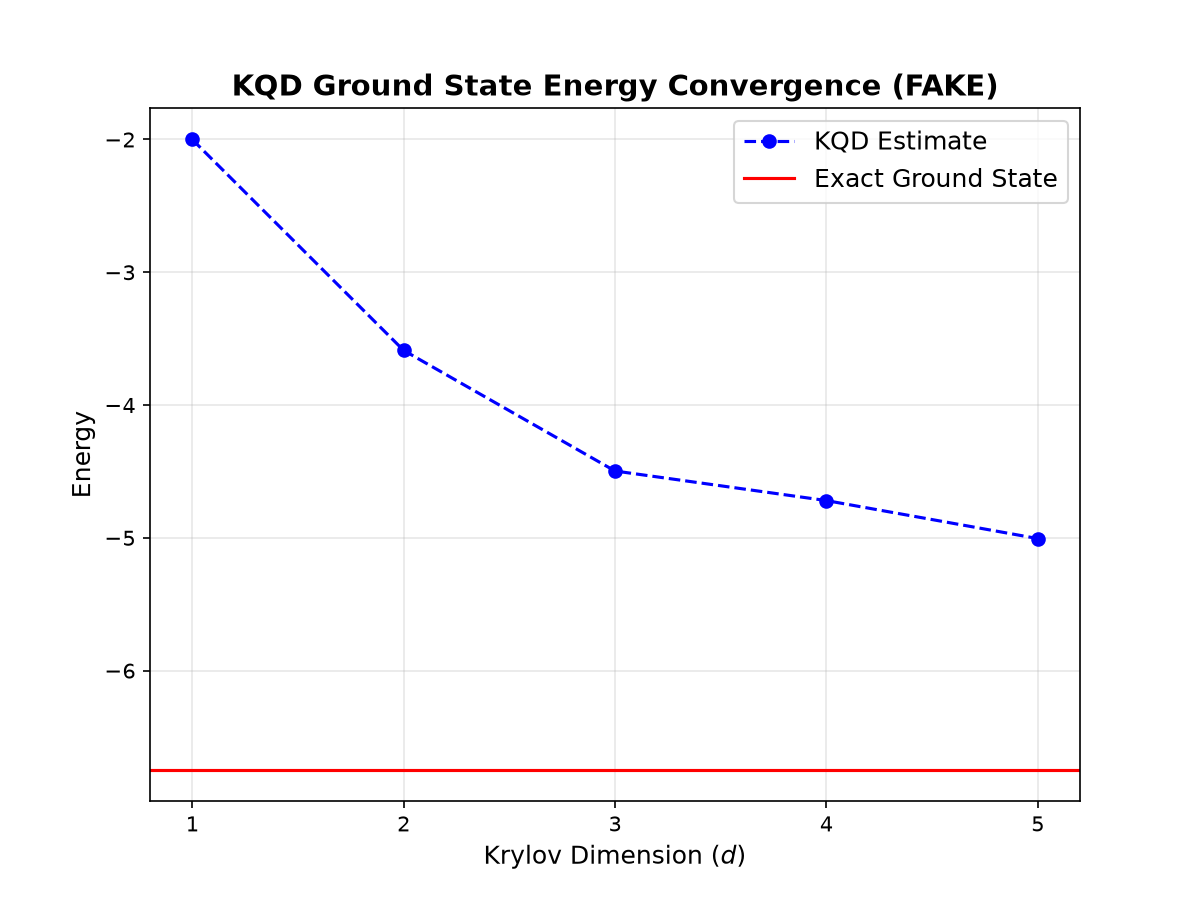
\includegraphics[width=0.7\textwidth]{kqd_convergence_fake.png}
\caption{KQD ground state energy convergence on the noisy FakeBrisbane simulator (2-step Lie Trotter, ZNE enabled). Despite noise, the KQD method converges to $-5.005$ at $d=5$, significantly better than unmitigated deep-circuit estimates.}
\label{fig:kqd_fake}
\end{figure}

\section{Conclusion}
KQD provides a major advantage on NISQ hardware by reducing the quantum circuit depth and gate counts, enabling effective error mitigation. While increasing Trotter steps improves convergence accuracy, it also increases circuit depth (from 17 to 52 for 1-step to 6-step), presenting a trade-off that must be tuned per application. Standard Trotterization time-domain data can be analyzed classically via FFT to extract energy transition frequencies without resorting to deep QPE circuits, providing complementary information to KQD's direct energy estimation. KQD remains an exceptionally robust algorithm for NISQ-era lattice Hamiltonian simulations.

\end{document}
